\section{Ejercicio 1}

\subsection{Introducción}
Este ejercicio consiste en entrenar una red neuronal que, dados los resultados de un examen específico que es utilizado en el diagnóstico del
cáncer de mamas, sepa clasificar ese conjunto dentro de dos categorias posibles: B y M. Para el este ejercicio B significará que el tumor diagnosticado
es benigno y M será maligno.

\subsection{Experimentación}
Al ser un ejercicio de clasificacion la red neuronal deberá devolver un valor para cada clase, por lo que la ultima función de activacion necesariamente
deberá devolver unicamente dos valores posibles. En este caso se utilizó la función signo bipolar, la cual devolvera -1 en caso de la muestra pertenecer
a la clase M (Maligno) y 1 en caso contrario la clase B (Benigno).

Tambien se decidió utilizar el 60\% de los datos como datos de entrenamiento y el 40\% restante como datos de validacion. Esta eleccion se debe a que
queremos poder extraer una mayor cantidad de informacion del entramiento, antes de pasar a clasificar nuevos datos.

\subsubsection{Experimento 1}
Este experimento consistió en comparar distintas arquitecturas de redes neuronales variando la cantidad de capas ocultas y de neuronas por capa.
Para este experimento se decidió fijar el coeficiente de aprendizaje $\eta$ en 0.03, la cantidad de epocas sobre las que se entrena la red en 1000 y el
método de entrenamiento estocástico. Con respecto a las funciones de activación se utilizaron sigmoideas para las capas intermedias y la función signo
para la capa final.

Las redes que se utilizaron fueron las siguientes:
\begin{enumerate}
  \item 10 - 1 (Perceptron simple): Esta red se planteó para ver si el problema era linealmente separable y podia ser aprendido por un perceptron
                                      simple.
  \item 10 - 20 - 1: Esta red se planteo para extraer una cantidad de features mayor a la cantidad de datos de entrada del problema y asi poder sintetizar
                      estos en la neurona de salida.
  \item 10 - 5 - 5 - 8 - 1: Esta red se planteo para analizar el comportamiento de la red al agregarle mas etapas de procesamiento anidadas.
\end{enumerate}

Los resultados que se obtuvieron fueron los siguientes:
\begin{figure}[h!]
  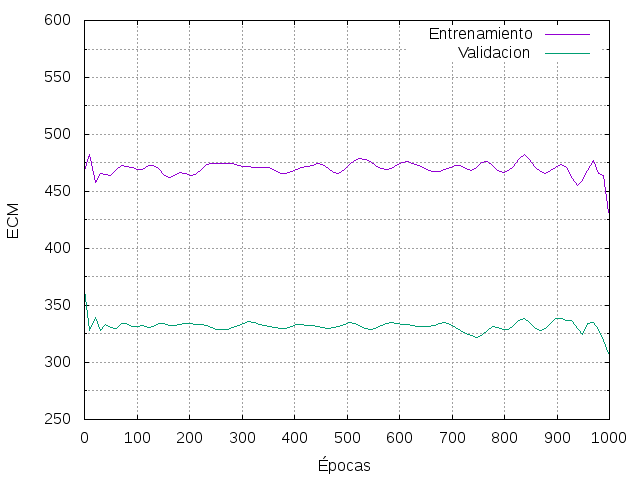
\includegraphics[width=125mm]{imagenes/ej1/ex_1-1_red_11-1_errors.png}
  \caption{Red 1}
\end{figure}

\begin{figure}[h!]
  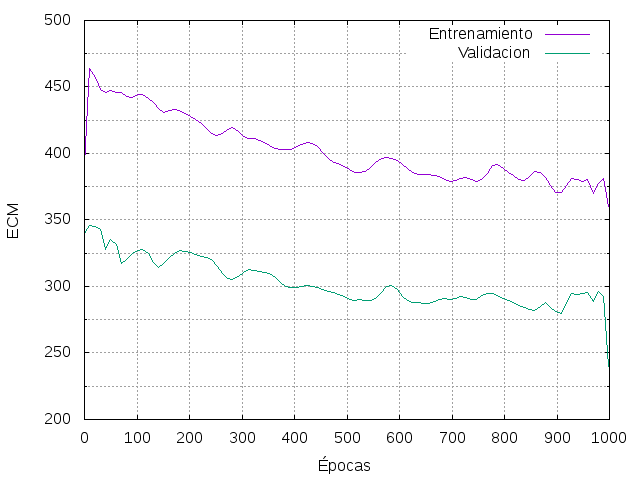
\includegraphics[width=125mm]{imagenes/ej1/ex_1-1_red_11-6-6-9-1_errors.png}
  \caption{Red 2}
\end{figure}

\begin{figure}[h!]
  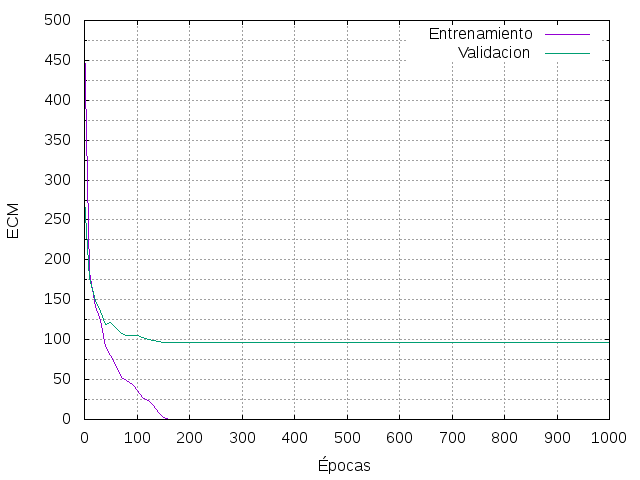
\includegraphics[width=125mm]{imagenes/ej1/ex_1-1_red_11-21-1_errors.png}
  \caption{Red 3}
\end{figure}


 Tal como se observa en los resultados de la Red 1, la cual es un perceptrón simple, el error cuadratico medio (ECM) no es notorio un decrecimiento (aun mas una oscilacion
 muy variada) de esta a medida que aumentan las epocas.
 Esto tambien se evidencia en la tabla de aciertos en la cual logra un 62.60\% de aciertos sobre los datos de entrenamiento y un 61.58\% sobre datos de validación,
 lo cual es bastante bajo siendo 1000 la cantidad de epocas con las que se entrena. Ademas analizando las columnas de falsos positivos y falsos negativos no se observó
 predominancia de un tipo de error sobre el otro, es decir que casi la mitad de las veces se observan falsos negativos, lo cual no es deseable para el dominio de este problema.
 Con toda la evidencia provista por los graficos se estimó que el problema a resolver no es linealmente separable pues no es posible
 aprenderlo con un perceptrón simple, por lo tanto esta red se descartó para futuros experimentos ya que sus resultados no fueron relevantes.

 Con respecto a la Red 2, se observa que el ECM decrece casi linealmente tanto en validacion como en entrenamiento, comenzando en 340 sobre validacion y
 logrando un valor minimo de 96. En la tabla de aciertos se observa un 99.59\% de aciertos sobre entrenamiento y un 89.02\% sobre validacion. Tambien se observa
 que el ritmo de aprendizaje es inferior con respecto a la Red 3 pero es superior al de la Red 1, sin embargo, dados los resultados obtenidos se consideró
 que puede ser notablemente mejorada con una optimizacion del algoritmo de BackPropagation, por lo que se decidió continuar experimentado sobre ella.

 Finalmente, la red 3 es la que mejor aprende de los datos de entrenamiento llegando al valor minimo absoluto de 0 en ECM sobre los datos de entrenamiento y un valor minimo
 de 96 en ECM sobre datos de validación. Tambien se observa que la funcion del ECM decrece rapidamente por lo que se concluye que este perceptron multicapa
 logra aprender en solo 150 epocas todo el set de entrenamiento. Esto trae como desventaja el hecho de que no se podrá disminuir mucho mas el ECM puesto que el set
 de entrenamiento fue completamente aprendido y luego de esto el ECM del set de validacion se mantendrá constante.
 A pesar de esto, en la tabla de aciertos se observó un alto
 porcentaje de aciertos, 100\% y 89.63\% para entrenamiento y validacion respectivamente por lo que se decidió seguir utilizando esta red para futuros experimentos
 con el objetivo de mejorar el porcentaje de aciertos sobre validacion al hacer mejoras al algoritmo de BackPropagation.

\subsubsection{Experimento 2}
Para este experimento se decidió variar el coeficiente de aprendizaje $\eta$ e introducir la optimizacion del \textit{momentum} al algoritmo de BackPropagation,
variando su respectivo parametro $\alpha$. Esto permite darle una aceleracion o decaiminento al nivel de aprendizaje en base al valor del parametro.
Las redes utilizadas fueron las redes 2 y 3 del Experimento 1, con 1000 epocas y continuando con el modo entrenamiento estocastico.
El valor de $\eta$ lo variamos con los siguientes valores: 0.03 y 0.07, mientras que el valor de $\alpha$ se varió con los valores: 0.1 y 0.3,
con lo cual se obtuvieron 4 combinaciones posibles para cada red. Estos valores se elegieron dentro de lo razonable (valores de $\eta$ mayores a 0.1
representan un cambio brusco en el aprdendizaje) para representar las posibles combinaciones de $\eta$ chico/grande junto a un $\alpha$ chico/grande y
 asi poder analizar diversos comportamientos de la red.

 Los resultados obtenidos se presentan a continuacion:

\begin{figure}[h!]
  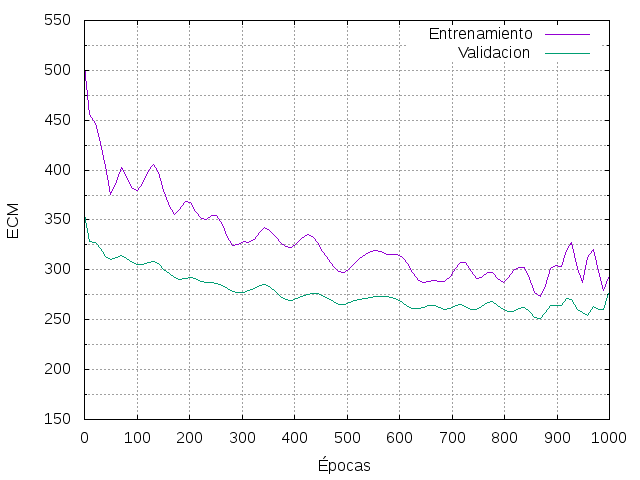
\includegraphics[width=125mm]{imagenes/ej1/ex_2-1_red_11-6-6-9-1_errors.png}
  \caption{Red 3 con parametros $\eta = 0.07$ y $  \alpha = 0.1$}
\end{figure}

\begin{figure}[h!]
  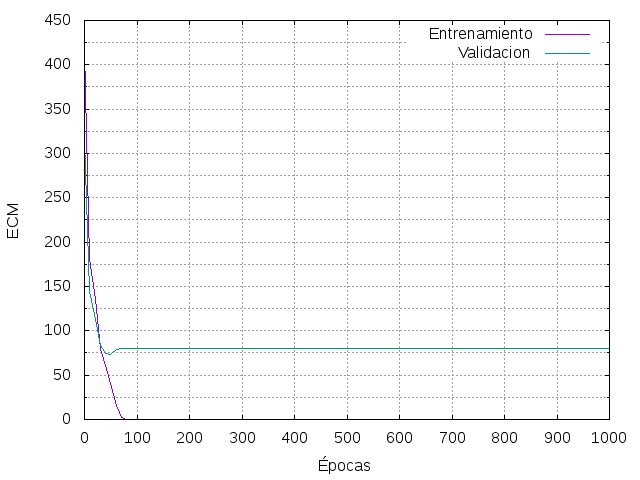
\includegraphics[width=125mm]{imagenes/ej1/ex_2-1_red_11-21-1_errors.png}
  \caption{Red 2 con parametros $\eta = 0.07$ y $  \alpha = 0.1$}
\end{figure}

\begin{figure}[h!]
  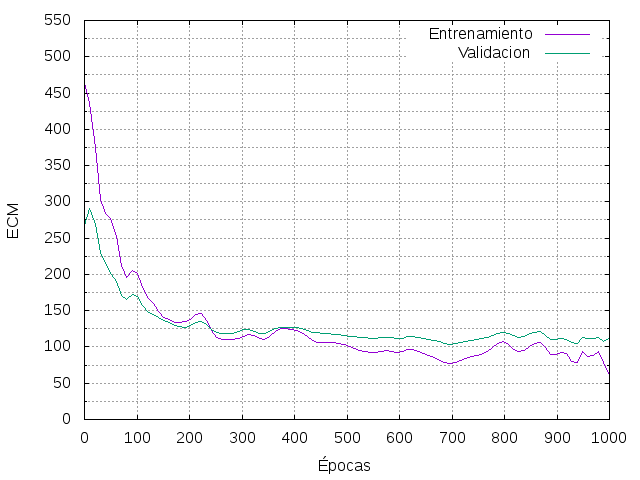
\includegraphics[width=125mm]{imagenes/ej1/ex_2-2_red_11-6-6-9-1_errors.png}
  \caption{Red 3 con parametros $\eta = 0.03$ y $\alpha = 0.1$}
\end{figure}

\begin{figure}[h!]
  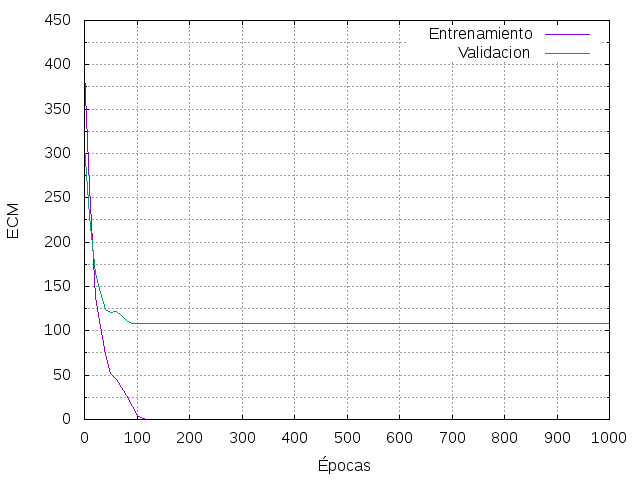
\includegraphics[width=125mm]{imagenes/ej1/ex_2-2_red_11-21-1_errors.png}
  \caption{Red 2 con parametros $\eta = 0.03$ y $  \alpha = 0.1$}
\end{figure}

\begin{figure}[h!]
  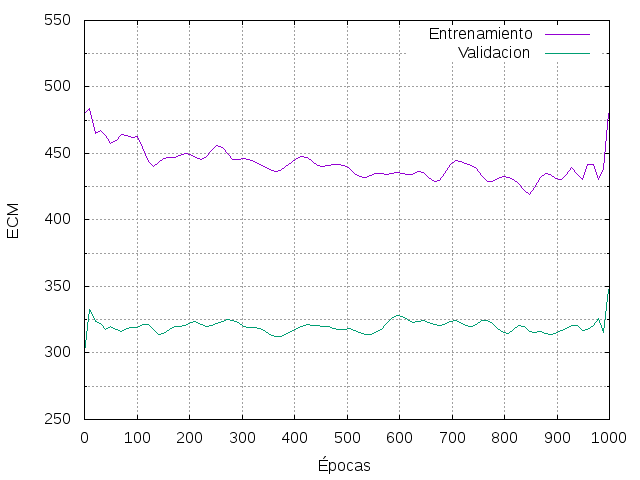
\includegraphics[width=125mm]{imagenes/ej1/ex_2-3_red_11-6-6-9-1_errors.png}
  \caption{Red 3 con parametros $\eta = 0.03 $ y $ \alpha = 0.3$}
\end{figure}

\begin{figure}[h!]
  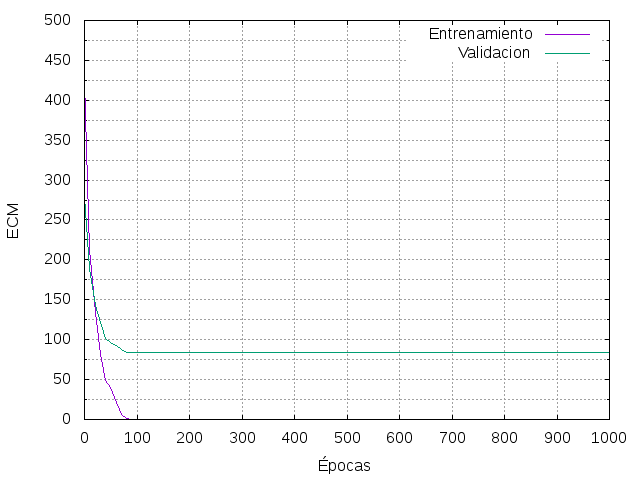
\includegraphics[width=125mm]{imagenes/ej1/ex_2-3_red_11-21-1_errors.png}
  \caption{Red 2 con parametros $\eta = 0.03 $ y $ \alpha = 0.3$}
\end{figure}

\begin{figure}[h!]
  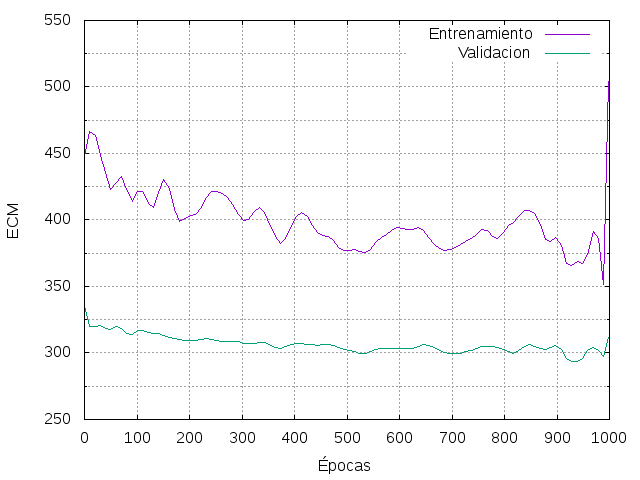
\includegraphics[width=125mm]{imagenes/ej1/ex_2-4_red_11-6-6-9-1_errors.png}
  \caption{Red 3 con parametros $\eta = 0.07 $ y $ \alpha = 0.3$}
\end{figure}

\begin{figure}[h!]
  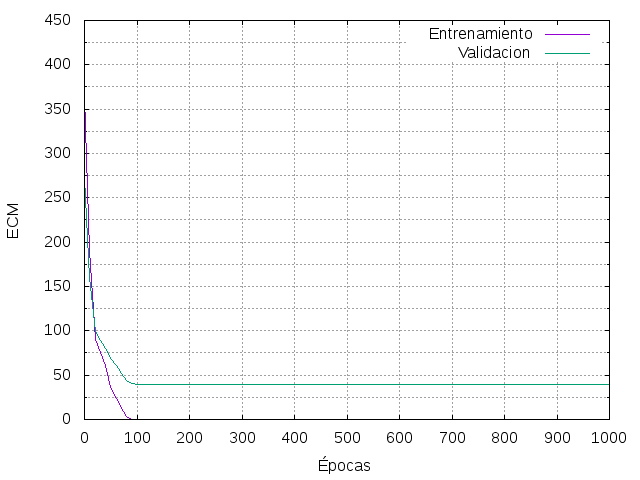
\includegraphics[width=125mm]{imagenes/ej1/ex_2-4_red_11-21-1_errors.png}
  \caption{Red 2 con parametros $\eta = 0.07 $ y $ \alpha = 0.3$}
\end{figure}

Se observa que la mejor combinacion de parametros para la Red 2, es aquella en la cual $\eta = 0.07$ y $\alpha = 0.3$, pues presenta los valores
mas bajos de ECM en validacion, alcanzando valores por debajo de 50. Con respecto a la cantidad de aciertos para estos parametros se obtiene un
93.90\% en datos de validacion y a su vez se obtiene la misma cantidad de falsos positivos como de falsos negativos en caso de fallos.
 Esto mejora ampliamente los resultados obtenidos en el experimento 1 y contradice el hecho de que el ECM no podia disminuir mas debido a la veloz
 convergencia.

Con respecto a la Red 3, la mejor combinacion de parametros fue $\eta = 0.03$ y $\alpha = 0.1$, en la cual se observan valores de ECM por debajo de 150
en validacion. Tambien se observa una mejora en la cantidad de aciertos obteniendo un valor de 88.41\%, esta mejora de un 20\% con respecto al experimento
anterior, validan la hipotesis de que esta red podia ser aun mas optimizada para poder competir con la eficiencia de la Red 2.


A raíz de estos experimentos se concluyó que para la Red 2 una mayor influencia de los pesos de las epocas anteriores genera una mejora en la performance
de esta red. En cambio, la Red 3 al agregar una minima proporcion de los pesos de las epocas anteriores genera una importante mejora en la eficiencia
de la red.
Finalmente para el resto de la experimentacion se decidio descartar la Red 2 debido a que obtuvo una mejora de solo un 3\% en la cantidad de aciertos,
mientras que la Red 3 obtuvo un 20\%.

\subsubsection{Experimento 3}
Para este experimento se decidió experimentar con parametros adaptativos y sus respectivos coeficientes $a$ y $b$. Se utilizó la Red 3 definida
previamente, fijando la cantidad de epocas en 1000, continuando aun con el modo de entrenamiento estocástico, $\eta = 0.03$ y $\alpha = 0.1$ ( producto
de los mejores parametros del experimento anterior).
Con respecto a los coeficientes de los parametros adaptativos, se fijo $a = 0.02$ y $b$ se varió con los valores: 0.7 y 0.1. La eleccion del $a$ se debe
a que en caso de disminuir el error se buscó aumentar el $\eta$, pero que la diferencia de salto no sea muy grande o se mantenga chica. Los valores de
 $b$ representan la disminucion de un porcentaje del valor del $\eta$ anterior, produciendo que los saltos sean mas finos, y es por esto que se decidió
 tomar un valor representantivo grande(0.7) y otro chico(0.1).

Los resultados obtenidos fueron los siguientes:
\begin{figure}[h!]
  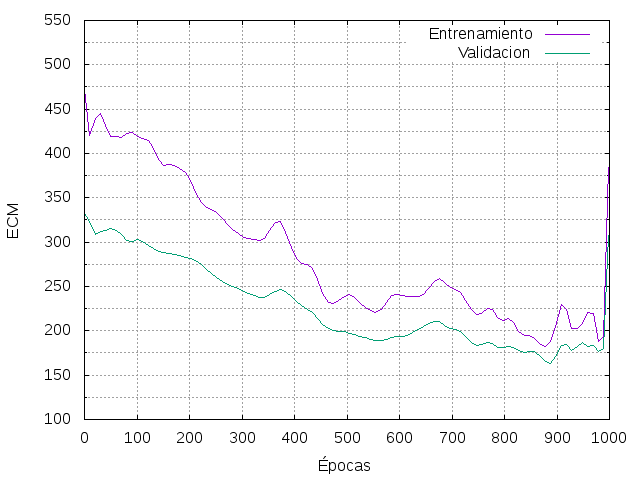
\includegraphics[width=125mm]{imagenes/ej1/ex_3-1_red_11-6-6-9-1_errors.png}
  \caption{Red 3 con parametros $a = 0.02 $ y $b= 0.7$}
\end{figure}

\begin{figure}[h!]
  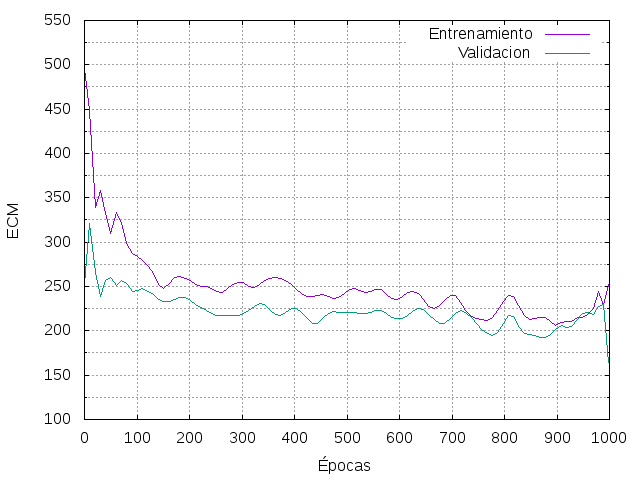
\includegraphics[width=125mm]{imagenes/ej1/ex_3-2_red_11-6-6-9-1_errors.png}
  \caption{Red 2 con parametros $a = 0.02 $ y $b = 0.1$}
\end{figure}

Sobre estos resultados no se observó una mejora con respecto a los obtenidos en el experimento anterior por lo cual estos parametros no serán
tenidos en cuenta para el resto de la experimentacion.

\subsubsection{Experimento 4}
Para este experimento se decidió variar el modo de entrenamiento entre \textit{Batch} y \textit{Mini Batch}. Para este ultimo se tomó como tamaño
de batch los valores 10 y 30. Con respecto a los valores restantes se utilizaron los mismos a la configuracion del Experimento 3.

Los resultados obtenidos fueron los siguientes:

\begin{figure}[h!]
  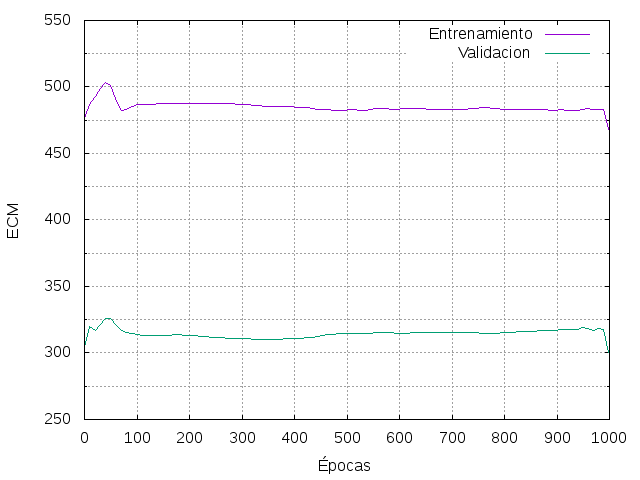
\includegraphics[width=125mm]{imagenes/ej1/ex_4-1_red_11-6-6-9-1_errors.png}
  \caption{Modo de entrenamiento Batch}
\end{figure}

\begin{figure}[h!]
  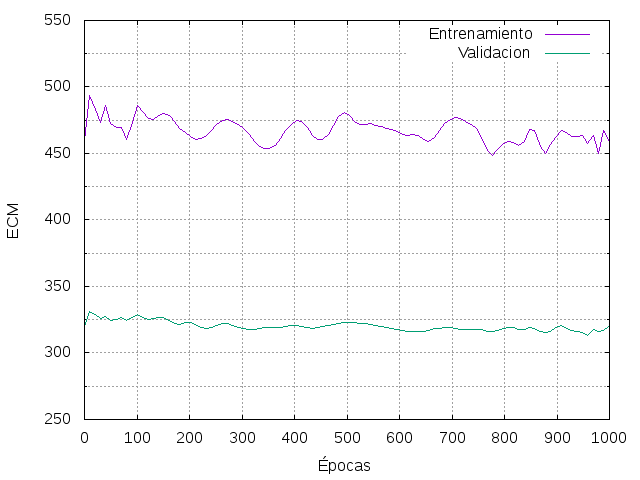
\includegraphics[width=125mm]{imagenes/ej1/ex_4-2_red_11-6-6-9-1_errors.png}
  \caption{Modo de entrenamiento Mini Batch con tamaño de batch 10}
\end{figure}

\begin{figure}[h!]
  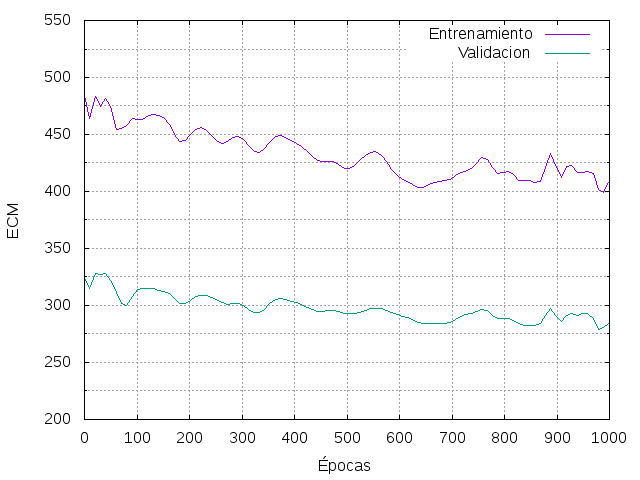
\includegraphics[width=125mm]{imagenes/ej1/ex_4-3_red_11-6-6-9-1_errors.png}
  \caption{Modo de entrenamiento Mini Batch con tamaño de batch 30}
\end{figure}

Se concluyó que esta experimentacion no mejora los resultados obtenidos en experimentos anteriores. Por lo tanto se decidió
mantener el modo de entrenamiento en estocastico, con el cual se obtuvieron los mejores resultados.

\subsection{Tabla de aciertos}
A continuación se presenta la tabla de aciertos con todos los resultados de la experimentación del ejercicio 1.
\clearpage
\begin{figure}
\begin{longtable}{ccccccccc}
	\hline
	Ex & R & $\eta$ & ME & EP & MPT & MPV & FP & FN \\
	\hline
	1 & 2 & 0.03 & E  &                                       & 99.59 (96 epochs)  & 89.02 (88 epochs)  & 33.33  & 66.66 \\
	\hline
	1 & 3 & 0.03 & E  &                                       & 66.66 (969 epochs) & 64.02 (916 epochs) & 35.59  & 64.40 \\
	\hline
	1 & 1 & 0.03 & E  &                                       & 62.60 (944 epochs) & 61.58 (394 epochs) & 44.44  & 55.55 \\
	\hline
	2 & 2 & 0.07 & E  & $\alpha$ = 0.1                        & 98.37 (55 epochs)  & 93.29 (50 epochs)  & 54.54  & 45.45 \\
	\hline
	2 & 3 & 0.07 & E  & $\alpha$ = 0.1                        & 80.89 (903 epochs) & 71.34 (795 epochs) & 80.85  & 19.14 \\
	\hline
	2 & 2 & 0.03 & E  & $\alpha$ = 0.1                        & 99.59 (54 epochs)  & 87.80 (49 epochs)  & 40.0   & 60.0 \\
	\hline
	2 & 3 & 0.03 & E  & $\alpha$ = 0.1                        & 96.34 (934 epochs) & 88.41 (577 epochs) & 52.63  & 47.36 \\
	\hline
	2 & 2 & 0.03 & E  & $\alpha$ = 0.3                        & 99.59 (58 epochs)  & 88.41 (43 epochs)  & 73.68  & 26.31 \\
	\hline
	2 & 3 & 0.03 & E  & $\alpha$ = 0.3                        & 64.22 (766 epochs) & 57.92 (685 epochs) & 5.79   & 94.20 \\
	\hline
	2 & 3 & 0.07 & E  & $\alpha$ = 0.3                        & 72.76 (818 epochs) & 60.97 (816 epochs) & 59.375 & 40.625 \\
	\hline
	2 & 2 & 0.07 & E  & $\alpha$ = 0.3                        & 99.59 (52 epochs)  & 93.90 (100 epochs) & 50.0   & 50.0 \\
	\hline
	3 & 3 & 0.03 & E  & \tcell{$\alpha$ = 0.1\\ $a$ = 0.02\\ $b$ = 0.7} & 88.61 (928 epochs) & 79.26 (880 epochs) & 50.0   & 50.0 \\
	\hline
	3 & 3 & 0.03 & E  & \tcell{$\alpha$ = 0.1\\ $a$ = 0.02\\ $b$ = 0.1} & 84.14 (968 epochs) & 79.87 (924 epochs) & 36.36  & 63.63 \\
	\hline
	4 & 3 & 0.03 & B  & $\alpha$ = 0.1                        & 52.84 (61 epochs)  & 58.53 (61 epochs)  & 2.94   & 97.05 \\
	\hline
	4 & 3 & 0.03 & MB & \tcell{b\_s = 10\\ $\alpha$ = 0.1}      & 65.85 (863 epochs) & 57.92 (239 epochs) & 89.85  & 10.14 \\
	\hline
	4 & 3 & 0.03 & MB & \tcell{b\_s = 50\\ $\alpha$ = 0.1}      & 71.54 (986 epochs) & 67.68 (827 epochs) & 35.84  & 64.15 \\
	\hline
\end{longtable}
\caption{\textbf{Columnas}:\\
         Ex: Experimento \\
         R: Nro de Red \\
         ME: Modo de Entrenamiento (E=Estocastico, B=Batch, MB=Mini-Batch)\\
         EP: Parametros Extras ($\alpha$=Momentum, $a$, $b$=Paratros adaptativos, b\_s=Tamaño del batch)\\
         MPT: Mejor \% de aciertos de Entrenamiento. Entre parsentesis en que época se alcanza\\
         MPV: Mejor \% de aciertos de Validacion. Entre parentesis en que época se alcanza\\
         FP: \% de Falsos Positivos en el error en validacion\\
         FN: \% de Falsos Negativos en el error en validacion}
\end{figure}



\subsection{Conclusión}

\newpage
